\documentclass{article}

\usepackage{multicol}
\usepackage{amsmath}
\usepackage{tikz}
\usetikzlibrary{bayesnet}

\setlength\columnsep{3cm}

\begin{document}

\begin{multicols}{2}
  \begin{align*}
    y_i &\sim Poisson(\lambda_i) \\
    ln(\lambda_i) &= a + \boldsymbol{x}_i\boldsymbol{\beta} + f_{c[i],g[i]} +
    \boldsymbol{z}_i\boldsymbol{\gamma} + \tilde{f}_{c[i],p[i],g[i]} \\
    \\
    a &\sim Unif(-\infty, \infty) \\
    \beta_k &\sim StudentT(3, 0, 1) \\
    \\
    \boldsymbol{\gamma} &\sim \mathcal{N}(\boldsymbol{0},
    diag(\boldsymbol{\sigma}) \: \boldsymbol{\Omega} \:
    diag(\boldsymbol{\sigma})) \\
    \boldsymbol{\Omega} &\sim LKJ(1) \\
    \sigma_m &\sim StudentT(3, 0, 2.5) \\
    \\
    \boldsymbol{f}_{c[i]} &\sim GP(\boldsymbol{0}, \boldsymbol{K_{\rho, \alpha}}) \\
    \rho &\sim InvGamma(10, 500) \\
    \alpha &\sim \mathcal{N}(0, 1) \\
    \\
    \boldsymbol{\tilde{f}}_{c[i],p[i]} &\sim
    GP(\boldsymbol{0}, \boldsymbol{K_{\tilde{\rho}, \tilde{\alpha}}}) \\
    \tilde{\rho} &\sim InvGamma(20, 600) \\
    \tilde{\alpha} &\sim \mathcal{N}(0, 1) \\
  \end{align*}
  
 \columnbreak
  
  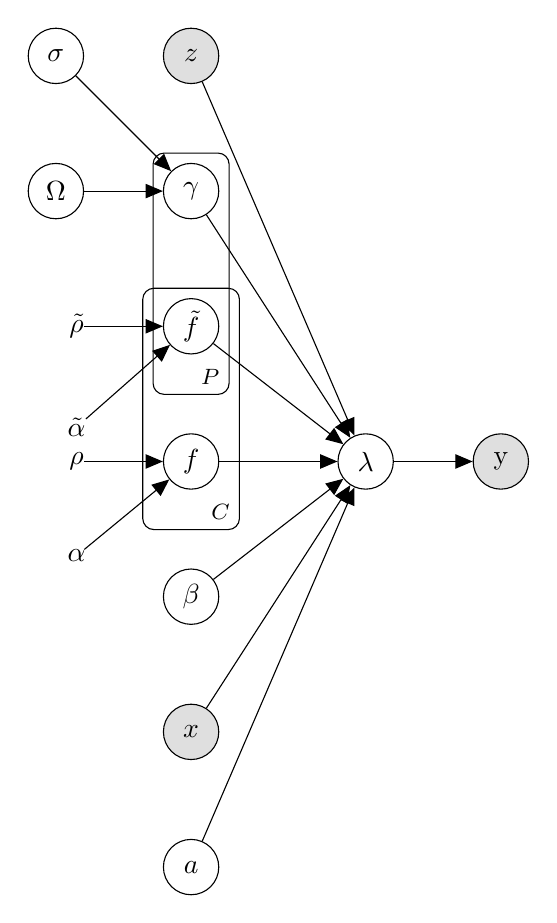
\begin{tikzpicture}
    \node[obs, yshift=1cm] (y) {y};
    \node[latent, left=of y] (lambda) {$\lambda$};
    \node[latent, left=of lambda, xshift=-0.5cm] (f) {$f$};
    \node[latent, above=of f] (ft) {$\tilde{f}$};
    \node[latent, above=of ft] (gamma) {$\gamma$};
    \node[obs, above=of gamma] (z) {$z$};
    \node[latent, below=of f] (beta) {$\beta$};
    \node[obs, below=of beta] (x) {$x$};
    \node[latent, below=of x] (a) {$a$};  
    
    \node[const, left=of ft] (rhot) {$\tilde{\rho}$};
    \node[const, below=of rhot] (alphat) {$\tilde{\alpha}$};
    \node[const, left=of f] (rho) {$\rho$};
    \node[const, below=of rho] (alpha) {$\alpha$};
    
    \node[latent, left=of gamma] (omega) {$\Omega$};
    \node[latent, above=of omega] (sigma) {$\sigma$};
    
    \edge {rho, alpha} {f};
    \edge {rhot, alphat} {ft};
    \edge {sigma, omega} {gamma};
    \edge {a, x, beta, z, gamma, ft, f} {lambda};
    \edge {lambda} {y};

    \plate {p} {(ft)(gamma)} {$P$};
    \plate {c} {(f)(ft)(p.south west)(p.south east)} {$C$};
  \end{tikzpicture}
  
\end{multicols}
\end{document}
